%
% problemstellung.tex -- Beispiel-File für die Beschreibung des Problems
%
% (c) 2020 Prof Dr Andreas Müller, Hochschule Rapperswil
%
\section{Problemstellung
\label{fem:section:problemstellung}}
\rhead{Problemstellung}
Für die Erklärung der Finiten Element Methode in der Ebene wird hier als Beispiel die folgende partielle Differentialgleichung (Poisson- Gleichung) mit dem Eigenwertproblem der Form 
\begin{equation}
	\Delta u = \lambda u
	\label{fem:equationPDE}
\end{equation}
verwendet, wobei der Laplace Operator die zweite Ableitungen nach den beiden Variablen darstellt:
\begin{equation}
	\Delta = \frac{\partial ^2}{\partial x^2} + \frac{\partial ^2}{\partial y^2}.
\end{equation} 
Diese PDE muss nach dem Abschnitt 7.1.1 auf einem definierten Gebiet z.B. ein Dreieck mit Werte am Rand $= 0$. Andere mögliche Randbedingungen sind in Abschnitt 7.1.3 zusammengestellt. Wie im Unterkapitel 7.4 behandelt, gibt es zu gewissen partiellen DGLen für ein Rechteck ein äquivalentes Minimalproblem.
\begin{equation}
	I(u) = \int_a^b \int_c^d \nabla u(x)^2 + \lambda u(x)^2 dy \, dx
	\label{fem:equationMinimalKapt7}
\end{equation}
Die Lösungsfunktion $u$ muss so gewählt werden, dass \eqref{fem:equationMinimalKapt7} minimal wird. Das Gebiet muss nicht zwinged ein Rechteck sein. Für ein beliebiges Gebiet $\Omega \subset \mathbb{R}^2$ wird das zu minimirende Integral  %Als vereinfachte Notation für ein Minimalproblem auf ein beliebiges Gebiet $\Omega$ für die PDA \eqref{fem:equationPDE} wird folgendes Integral aufgeschrieben:
\begin{equation}
	I(u) = \int_{\Omega} \nabla u(x)^2 + \lambda u(x)^2 dy \, dx
	\label{fem:equationMinimalKapt7Alg}
\end{equation}
geschrieben.
\subsection{Was sind Ansatzfunktionen?}
Um eine gesuchte Funktion $u(x,y)$ als Lösung für die partielle DGL \eqref{fem:equationPDE} zu finden, wird diese mit einfacheren Funktionen approximiert. Diese einfacheren Approximationsfunktionen werden in diesem Kapitel als Ansatzfunktion $u(x,y)$ bezeichnet..

Als einfachere Funktionen bieten sich Polynome mit niedrigem Grad an. Diese sind einfach integrier- und differenzierbar. Während der Polynomgrad 1 sehr leicht zu berechnen ist muss beim Polynomgrad 2 aufwändigere, aber nicht komplexere, Berechnungen durchgeführt werden, da quadratische Ausdrücke und davon Kombinationen entstehen. Polynomgrade 3 und 4 sind mit noch mehr Fleissarbeit verbunden, bieten dafür eine bessere Approximation an. Wie im Kapitel 7 ist auch hier das Ziel Gleichungen mit wenigen Unbekannten aufzustellen. Ist es möglich auch in der Ebene Ansatzfunktionen zu finden mit wenigen Koeffizienten, obwohl über ein Gebiet integriert wird? Es ist möglich, allerdings gibt es besondere Herausforderungen zu beachten, die in den nächsten Abschnitten genauer beschrieben werden.
%Die Ansatzfunktion ist frei wählbar und gibt auch den Freiheitsgrad vor. Je höher die Ordnung der Ansatzfunktion desto besser soll die Approximation werden. So die Hoffnung. Allerdings hat dies auch Konsequenzen, die im Verlauf dieses Kapitels beschrieben werden. 


\subsection{Herausforderung FEM in der Ebene}
Die einzelne lineare Ansatzfunktion kann nicht die globale Lösung sein. Ansonsten würde gemäss der Formel \eqref{fem:equationMinimalKapt7Alg}, die 2. differenzierbarkeit fordert, als einzige Lösung 0 zustande kommen, da lineare Terme als 2. Ableitung 0 aufweisen. Diese Lösung ist nicht sehr spannend. Daher muss das Gebiet $\Omega$ in Teilgebiete $\Omega_i$ unterteilt werden. Dadurch wird die Formel \eqref{fem:equationMinimalKapt7Alg} zu
\begin{equation}
\int_{\Omega} \nabla u(x)^2 + \lambda u(x)^2 \, dx \, dy = \sum \limits_{i=1}^n \int_{\Omega_i} \nabla u(x)^2 + \lambda u(x)^2 \, dx \, dy \, .
\label{fem:equationSummGebiete}
\end{equation}
Die Lösung verwendet das äquivalente Minimalproblem, also Integrale anstatt Ableitungen der Unbekannten. Entsprechend dem Kapitel 7 sind die Integrale von quadratischen oder linearen Ausdrücken. Das Prinzip der FEM in zwei Dimensionen wird hier anhand von linearen Ausdrücken erläutert. Das Prinzip ist für quadratische Ausdrücke genau gleich, lediglich die Berechnung ist mit mehr Aufwand verbunden. Die Integrale werden dann auf jedes Teilgebiet angewendet. \\
Damit eine Lösung gefunden werden kann, das Minimum über alle Teilgebiete zusammen zu finden, müssen die Teilgebiete einfach sein. Eine Approximation eines Gebietes kann beispielsweise mit Dreiecken, Rechtecken oder Parallelogrammen vorgenommen werden. Die Teilgebiete sind einfache geometrische Formen wie z.B. in Abbildung \ref{fig:Figuren}. Unterschiedliche geometrische Formen approximieren unterschiedlich gut das gewünschte Gebiet. Die Approximation mit Parallelogrammen z.B. deckt im Unterschied zu den anderen Approximationen das Gebiet weniger genau ab. Die Vierecke haben im Gegensatz zu den Dreiecken eine Unbekannte mehr bzw. einen Koeffzienten mehr der bestimmt werden  muss.
%Wie auch in der Dimension 1 wird das gesamte Gebiet $\Omega$ in Teilgebiete $\Omega_i$ unterteilt, damit einfache Formel entstehen können. Die einzelne Ansatzfunktion ist jedoch keine globale Lösung sondern alle Ansatzfunktionen zusammen stellen eine Lösung der Approximation dar. Die Teilgebiete sind einfache geometrische Formen wie z.B. in Abbildung \ref{fig:Figuren}. Unterschiedliche geometrische Formen approximieren unterschiedlich gut die gewünschte Fläche. Die Approximation mit Parallelogrammen z.B.  deckt im Unterschied zu den anderen Approximationen die Fläche weniger genau ab. Die Vierecke haben im Gegensatz zu den Dreiecken eine Unbekannte mehr bzw. einen Koeffzienten mehr der bestimmt werden  muss.
%Als Lösung dienen äquivalente Minimalprobleme sprich anstatt Ableitungen werden Integrale verwendet gemäss Kapitel 7.
\begin{figure}[h!]
	\centering
	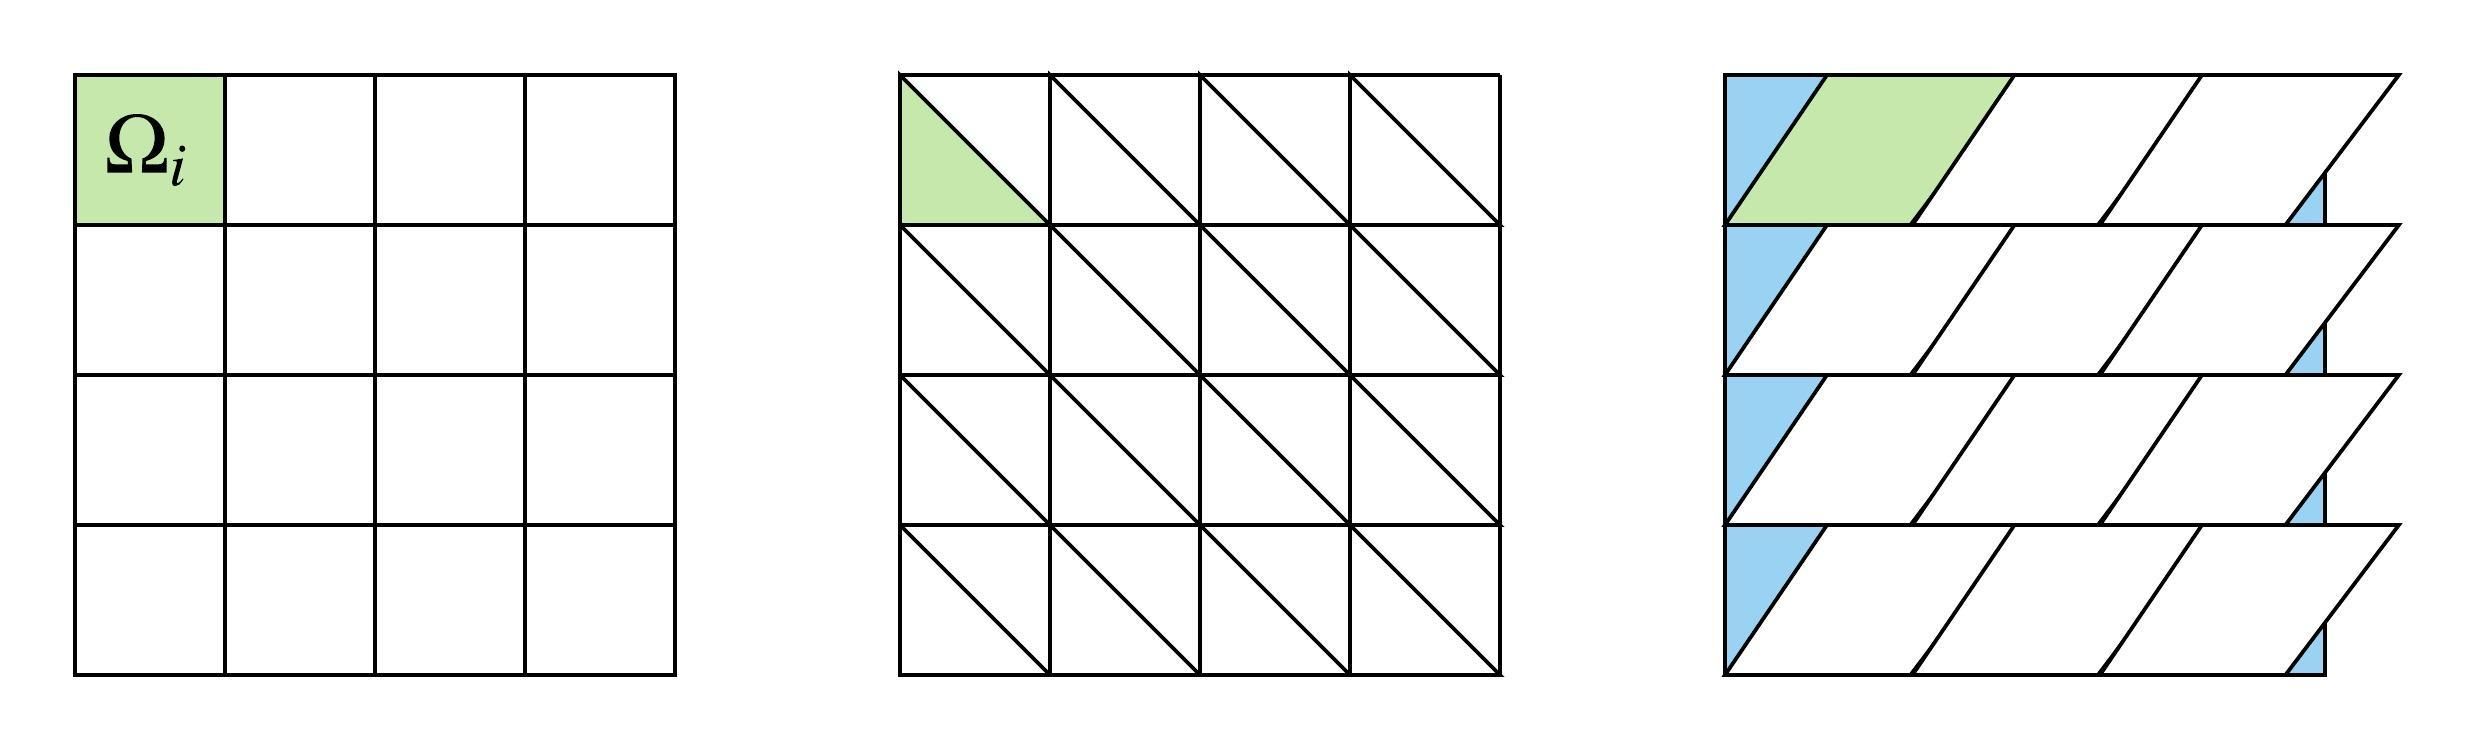
\includegraphics[scale=0.6]{papers/fem/Images/Figuren.jpeg}
	\caption{Approximationsmöglichkeiten eines Qudratischen Gebietes}
	\label{fig:Figuren}
\end{figure}

In einem nächsten Schritt muss die die approximierende Funktion betrachtet werden. Aus der Approximation resultieren zwei wesentliche Herausforderungen:
\begin{enumerate}
	\item Ansatzfunktion muss stetig differenzierbar in den Stützstellen (Steigung) sein wie z.B: im Dreieck in den Ecken.
	\item stetig differenzierbar an den Übergängen entlang den Rändern eines Elements zum anliegenden Rand eines benachbarten Elements. (Krümmung)
\end{enumerate}
Um diese beiden Herausforderungen etwas besser verständlich zu machen wurde  eine Funktion- Approximation dargestellt  $u(x,y) = 1-x^2-y^2$, welche eine Lösung der PDE $\Delta u = -4$ ist mit Randbedingungen $u=0$ auf dem Einheitskreis (violett).
\begin{figure}[h]
	\centering
	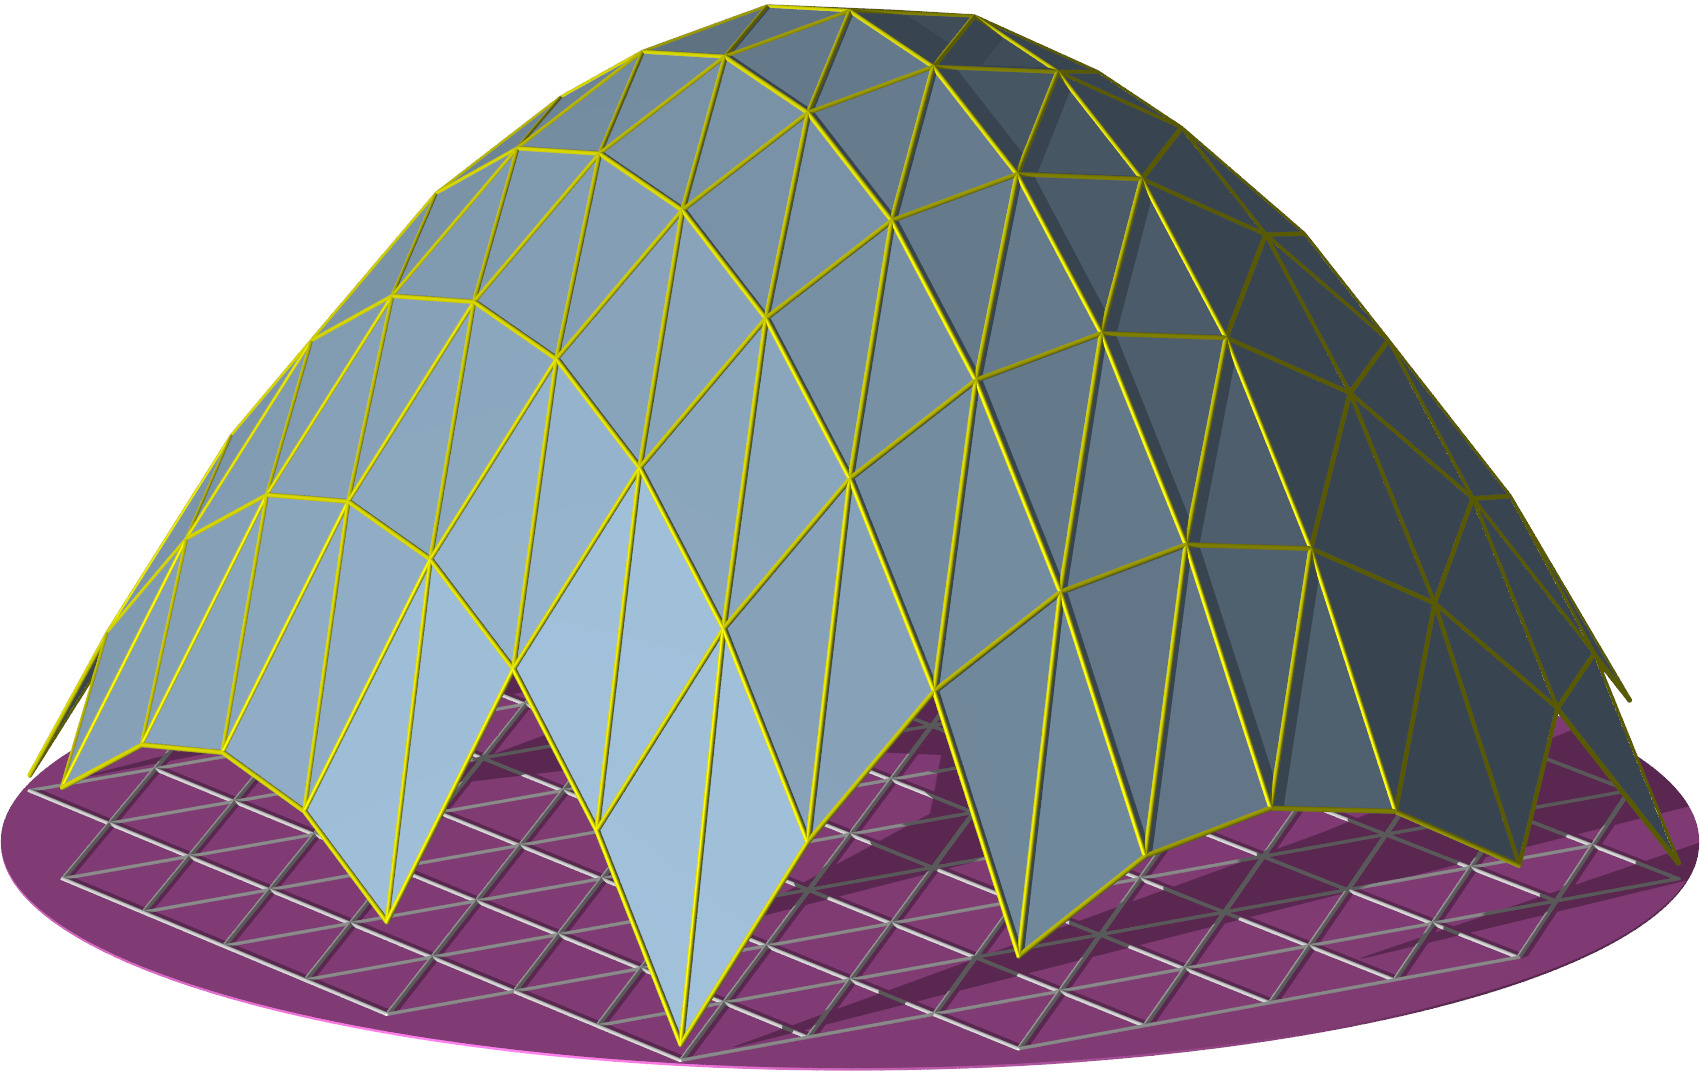
\includegraphics[scale=0.8]{papers/fem/Images/ansatz.jpg}
	\caption{Approximation mit Dreiecken auf einem quadratischen Gitter }
	\label{fig:Ansatz}
\end{figure}
Wie in der Abbildung \ref{fig:Ansatz} zu erkennen ist, passt die Approximation mit Dreiecken auf einem quadratischen Gitter nicht gut, da sich die Randbedingungen nicht ausnutzen lassen. Es benötigt also eine Unterteilung der Kreisscheibe die bis an den Rand kommt. Eine bessere Approximation ist in \ref{fig:besser Approx} zu sehen, die eine bessere Triangulation zeigt.
\begin{figure}[h!]
	\centering
	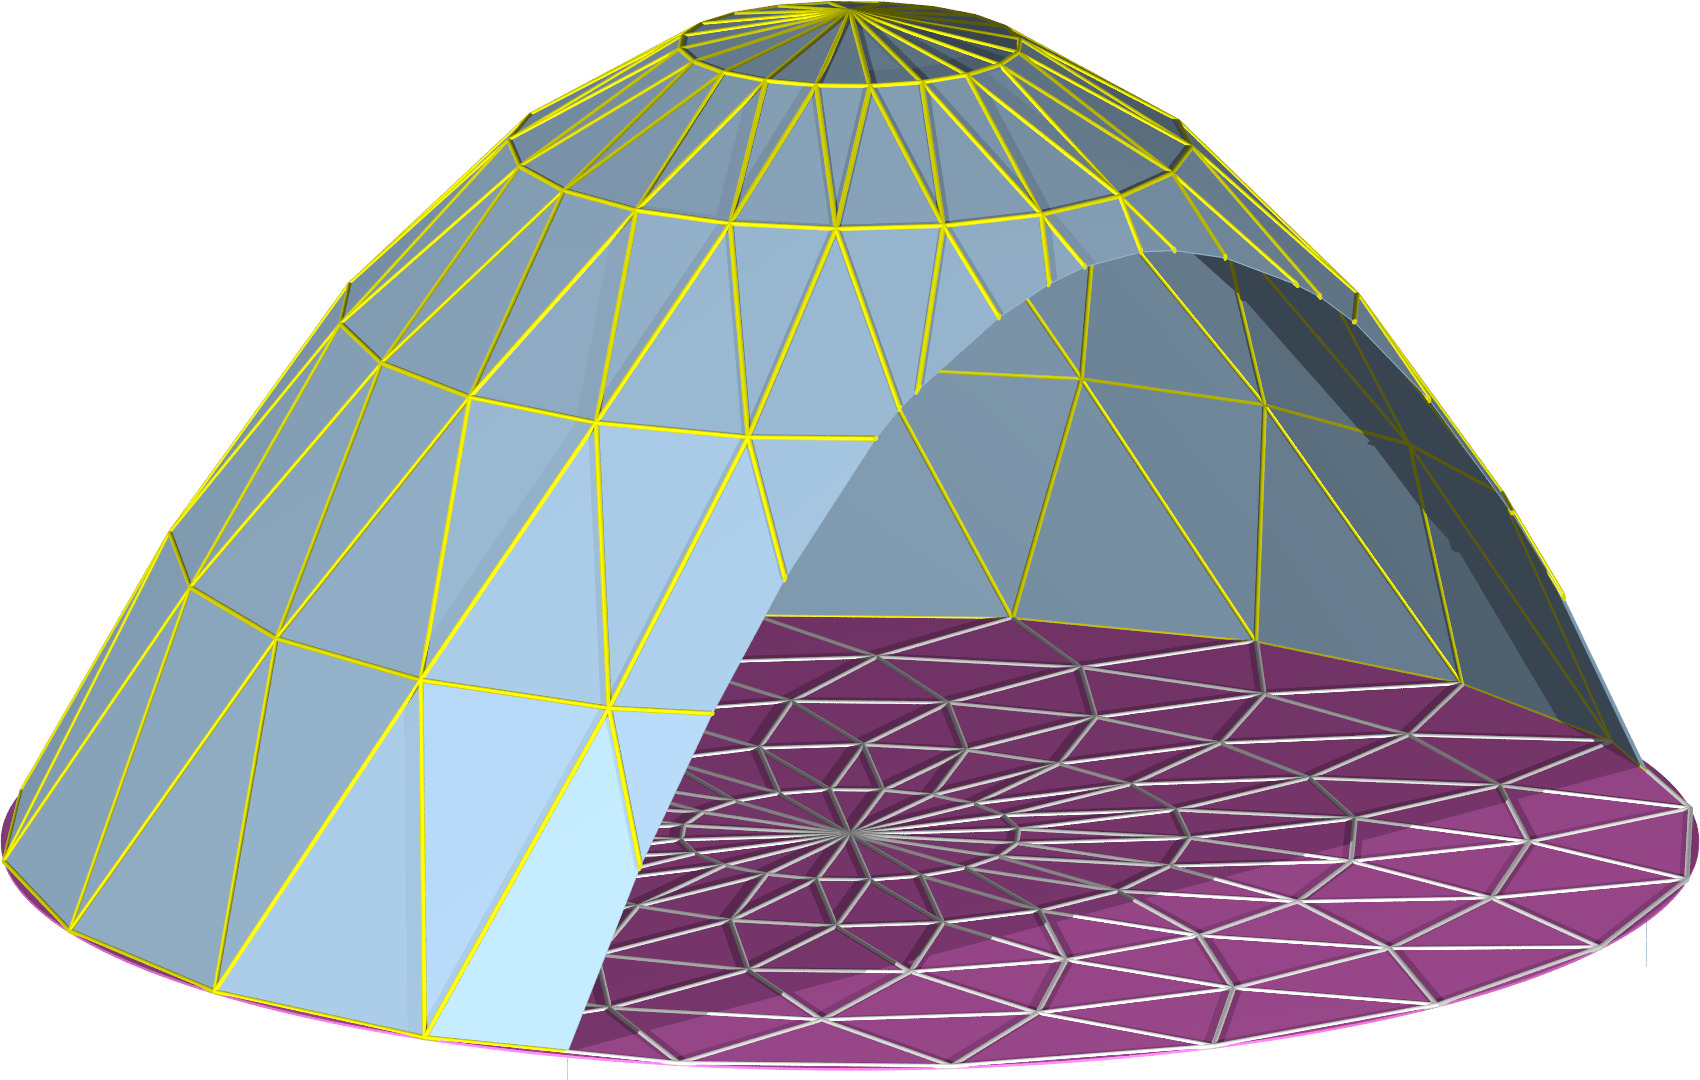
\includegraphics[scale=0.8]{papers/fem/Images/polar.jpg}
	\caption{bessere Triangulation}
	\label{fig:besser Approx}
\end{figure}
\begin{figure}[h]
	\centering
	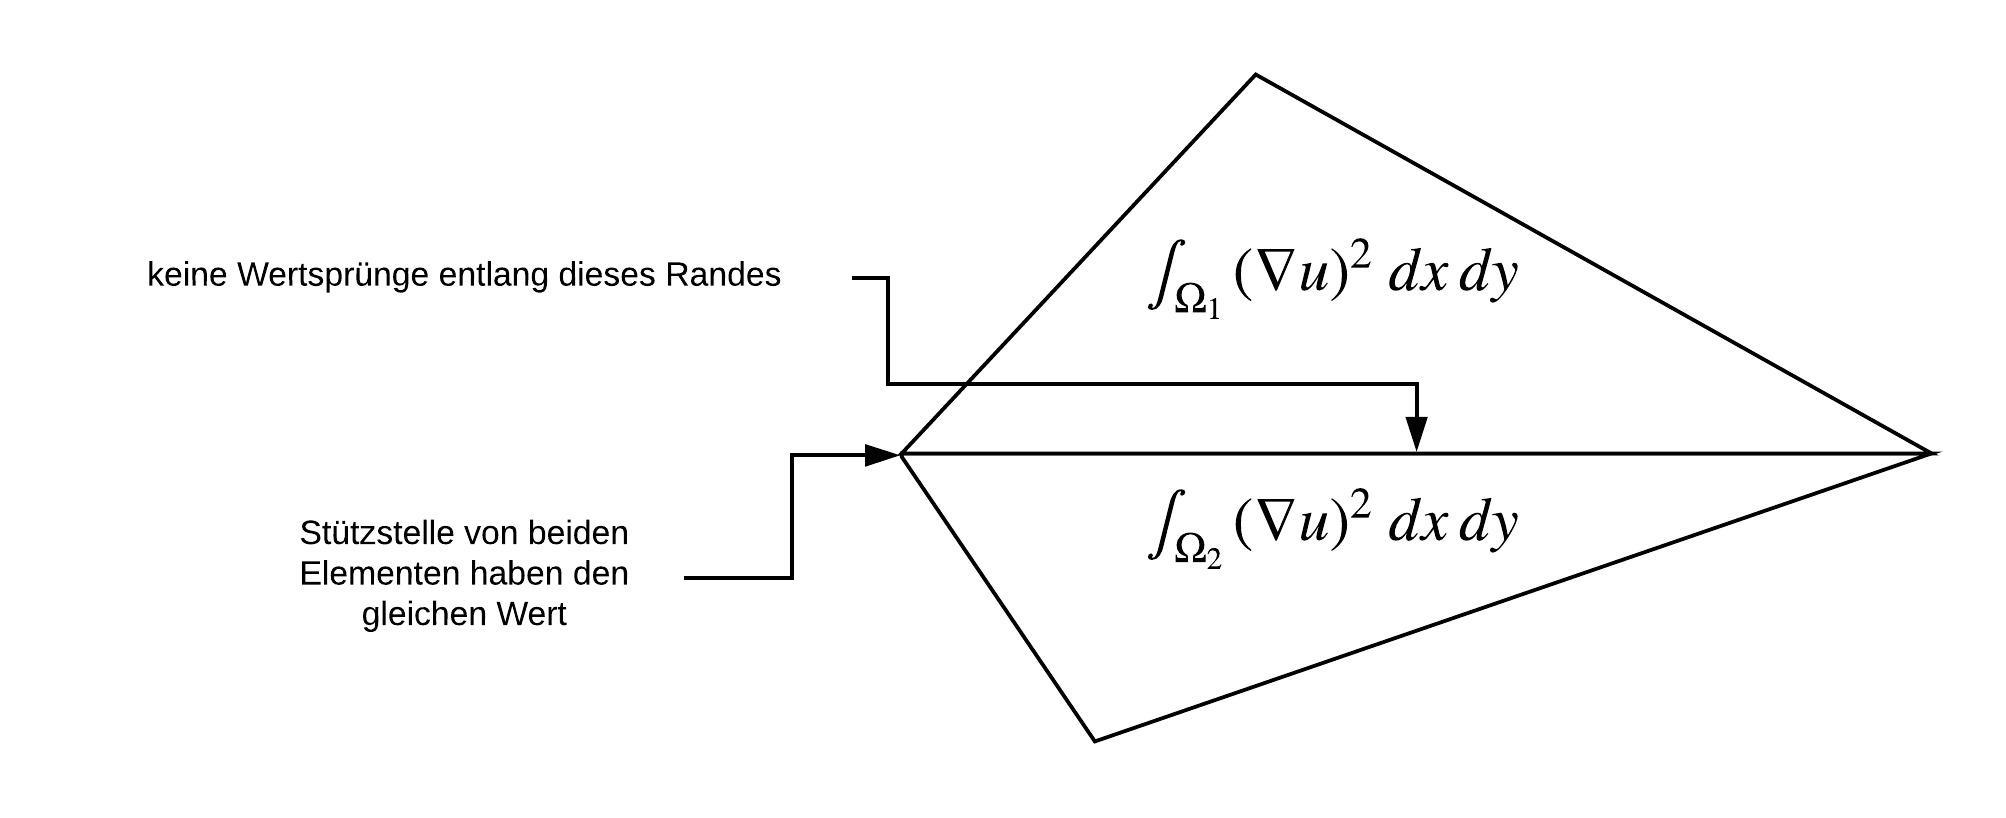
\includegraphics[scale=0.8]{papers/fem/Images/Rand.jpeg}
	\caption{differenzierbar entlang eines Randes}
	\label{fig:Randbedingung}
\end{figure}
Aus der Abbildung \ref{fig:besser Approx} lässt sich erkennen, dass die Ansatzfunktion für jedes Dreieck unterschiedlich ist. Auch müssen die Ansatzfunktionen flexibel auf die Grösse des Flächenelements anwendbar sein. Die Knicke von 2 benachbarten Elementen wird ignoriert, um das Lösungsvorgehen verständlicher aufzuzeigen. Bessere Ansatzfunktionen ergeben bessere Lösungen, aber die Vorgehensweise zu den linearen Gleichungen ist analog.
%Unteschiedlich zeigt sich im Vergleich der Differential Gleichung mit 1 Dimension und 2 Dimensionen. Die DGL wird folgender massen geändert 
%\begin{equation}
%	u'' = \lambda u \rightarrow \Delta u = \lambda u 
%	\label{fem:DGL2D}
%\end{equation} 
%während der Laplace Operator die 2. Ableitungen nach den beiden Variablen darstellt.
Aus den Integralen der Teilgebiete muss dann die Lösung gefunden werden, um die Koeffizienten in den Ecken zu bestimmen. Um den Aufwand der Berechnung über das Flächenelement zu minimieren wird in Abschnitt \ref{fem:section:loesung} auch eine Lösung aufgezeigt wie mit Hilfe einer Transformation das Dreiecks Flächenelement in ein weniger aufwändigeres berechenbare Flächenelement überführt werden kann.
Nochmals kurz zusammengefasst was bis hier hin aufgezeigt wurde.
\begin{itemize}
	\item Ebene wird in Teilgebiete unterteilt
	\item Teilgebiete können Dreiecke, Rechtecke oder Parallelogramme sein
	\item Ansatzfunktion soll ein Polynom nierigen Gerades sein
	\item auf jedes Teilgebiet wird eine Ansatzfunktion angewendet
\end{itemize} 
Was bis jetzt noch nicht klar ist, wie die Ansatzfunktion sich zusammenstellt. Dies wird under anderem im folgenden Abschnitt beschrieben.

%\subsection{De finibus bonorum et malorum
%\label{fem:subsection:finibus}}

%\begin{equation}
%\int_a^b x^2\, dx
%=
%\left[ \frac13 x^3 \right]_a^b
%=
%\frac{b^3-a^3}3.
%\label{fem:equation1}
%\end{equation}



